\clearpage
\section{Características técnicas del sistema}
\subsection{Alcance funcional y arquitectura}
El producto es un \textbf{servicio de información institucional}, compuesto por gestión editorial, consulta pública, distribución y continuidad. El piloto comprende tres terminales interiores de 55 pulgadas, red local de siete enlaces, videovigilancia de los terminales, CMS y cliente, contenido inicial, respaldo, subsistema FV, instalación, pruebas, capacitación y documentación. No incluye ampliar a toda la universidad, remodelación general, gestión de trámites con datos personales ni reemplazo de sistemas académicos.

La plataforma utilizará una administración central y clientes identificados por terminal y grupo. Se separarán publicación, consulta y supervisión mediante interfaces documentadas, con una base de datos y repositorio de medios respaldados. Esta arquitectura modular permite ampliar destinos y sustituir clientes sin rediseñar la gestión editorial.

\begin{center}
\begin{tikzpicture}[node distance=6mm,>=Latex,every node/.style={font=\small,align=center},box/.style={draw,rounded corners=2pt,text width=12.7cm,inner sep=6pt}]
\node[box] (f) {Fuentes autorizadas y emisores de la escuela\\Aviso, vínculo oficial, responsable e inicio/vencimiento};
\node[box,below=of f] (c) {CMS: borrador, revisión, aprobación y programación\\Cuentas individuales, permisos y registro de cambios};
\node[box,below=of c] (d) {Distribución de paquetes por versión y terminal\\Medios, vigencia, destino y confirmación de recepción};
\node[box,below=of d] (t) {Tres clientes públicos en modo kiosco\\Consulta táctil, QR, copia local y retorno al inicio};
\node[box,below=of t] (m) {Supervisión y continuidad\\Última comunicación, versión, incidencias y recuperación};
\draw[->](f)--(c);\draw[->](c)--(d);\draw[->](d)--(t);\draw[<->](t)--(m);
\end{tikzpicture}
\captionof{figure}{Arquitectura funcional del servicio de información}
\label{fig:arquitectura}
\end{center}

\subsection{Proceso editorial y modelo de información}
Cada aviso tendrá identificador, título, categoría, emisor, fuente oficial, texto o medio, inicio, vencimiento, destino y versión. La operación distinguirá contenido en borrador, en revisión, aprobado, publicado, vencido y retirado. El editor preparará; el revisor comprobará fuente y vigencia; el sistema publicará sólo la versión autorizada.

La primera operación utilizará carga validada de fuentes oficiales. Cada integración automática requerirá titular, autorización, formato, frecuencia, autenticación, campos y manejo de errores. La versión y la fuente del aviso permitirán rastrear su publicación y retirada.

El cuadro \ref{tab:fuentes_contenido} identifica de dónde procede cada tipo de información, quién la entrega y cómo ingresa al servicio. Los emisores son propuestos y la dirección de escuela los designará antes de la puesta en servicio.

\cuadro{tab:fuentes_contenido}{Origen, emisor y forma de ingreso de la información publicada}{@{}P{2.7cm}P{3.6cm}Y P{2.0cm}@{}}{\textbf{Información}&\textbf{Fuente oficial y emisor propuesto}&\textbf{Forma de ingreso y control}&\textbf{Vigencia}}{
Trámites y calendario & Dirección de escuela y secretaría académica; calendario y resoluciones de la universidad & El editor transcribe el aviso y enlaza el documento oficial; revisión antes de publicar & Hasta la fecha límite\\*
Becas y créditos & Unidades de bienestar y oficinas de becas; convocatorias oficiales externas & Aviso con enlace a la convocatoria y fecha de cierre; dato exigido por el art. 11.4 & Hasta el cierre\\
Eventos y capacitación & Escuela, centro federado y unidades organizadoras & Formulario interno del emisor y aprobación del revisor & Hasta el evento\\
Oportunidades profesionales & Convenios, prácticas y bolsa de trabajo de la universidad & Sólo ofertas con entidad identificada y enlace verificable & Hasta la postulación\\
Investigación y proyectos & Docentes responsables y grupos de investigación & Ficha autorizada por el titular; sin datos personales no consentidos & Semestral\\
Avisos urgentes & Dirección de escuela & Publicación prioritaria con doble verificación y retiro programado & Horas o días\\
}
El servicio no genera información propia ni reemplaza el documento oficial. Muestra un resumen verificable y el QR al documento de origen. Cuando una fuente se integre de forma automática, su formato y frecuencia se acordarán con el titular, conforme al requisito RF09.

\cuadro{tab:requisitos}{Requisitos funcionales y evidencia de aceptación}{@{}P{1.0cm}P{3.1cm}Y@{}}{\textbf{ID}&\textbf{Función}&\textbf{Criterio verificable}}{
RF01 & Consulta pública & Buscar categorías y abrir detalle; fuente y vigencia visibles, sin cuenta del estudiante\\*
RF02 & Edición y aprobación & Crear, revisar y programar; impedir publicación sin campos y autorización requeridos\\
RF03 & Destinos & Publicar en una, varias o todas las terminales; confirmar versión aplicada\\
RF04 & Caducidad & Retirar o advertir avisos vencidos, incluso bajo la política local de contingencia\\
RF05 & Consulta QR & Abrir vínculo institucional desde móvil; no encerrar información sólo en el edificio\\
RF06 & Continuidad & Conservar paquete aprobado y recuperar consulta tras corte de red y reinicio\\
RF07 & Supervisión & Registrar última comunicación, versión y errores; generar y asignar incidencia\\
RF08 & Auditoría & Conservar autor, revisor, fecha y cambios; exportar registro autorizado\\
RF09 & Integración condicionada & Validar esquema y permisos antes de consumir fuentes automáticas\\
}
Se priorizan RF01 a RF08. Las funciones de colaboración difundirán proyectos y contactos autorizados. RF09 se incorporará después de acreditar acceso e interoperabilidad con la fuente institucional.

\subsection{Experiencia de consulta e interfaz}
La consulta se organiza por oportunidades, eventos, trámites, información académica y proyectos de colaboración. Cada detalle mostrará fuente, fecha y vigencia; un código QR permitirá continuar la lectura en móvil. El inicio recuperará una vista simple tras inactividad y evitará formularios con datos personales en la terminal pública.
\begin{center}
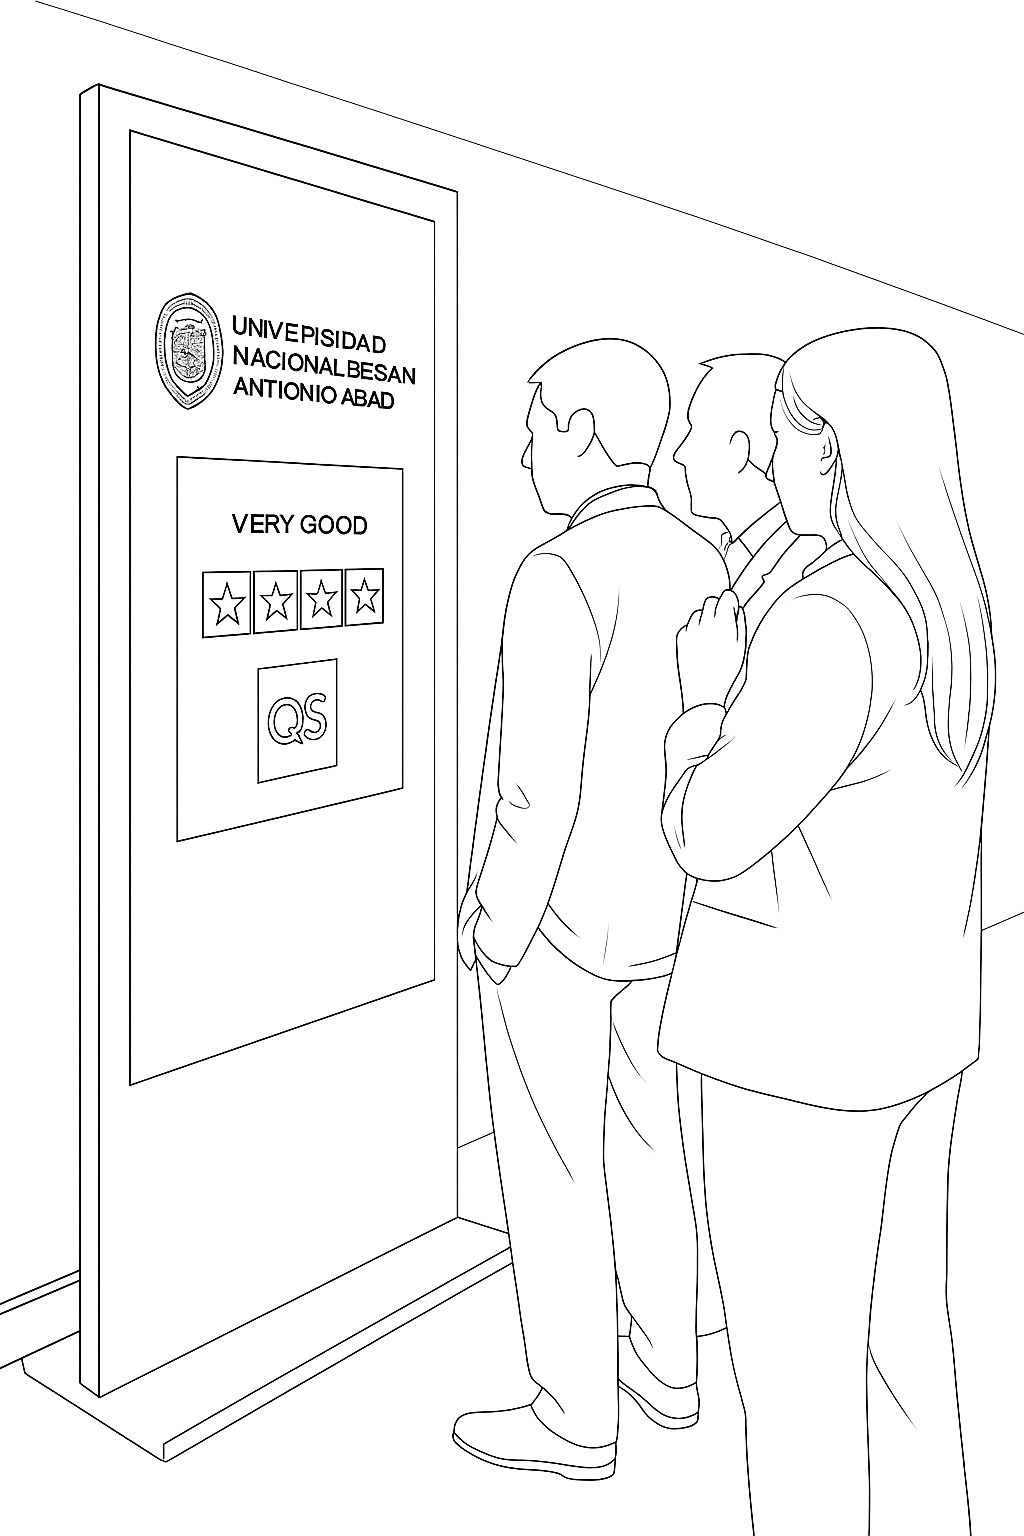
\includegraphics[width=0.47\linewidth,height=12cm,keepaspectratio]{imagenes/concepto_terminal.png}\hfill
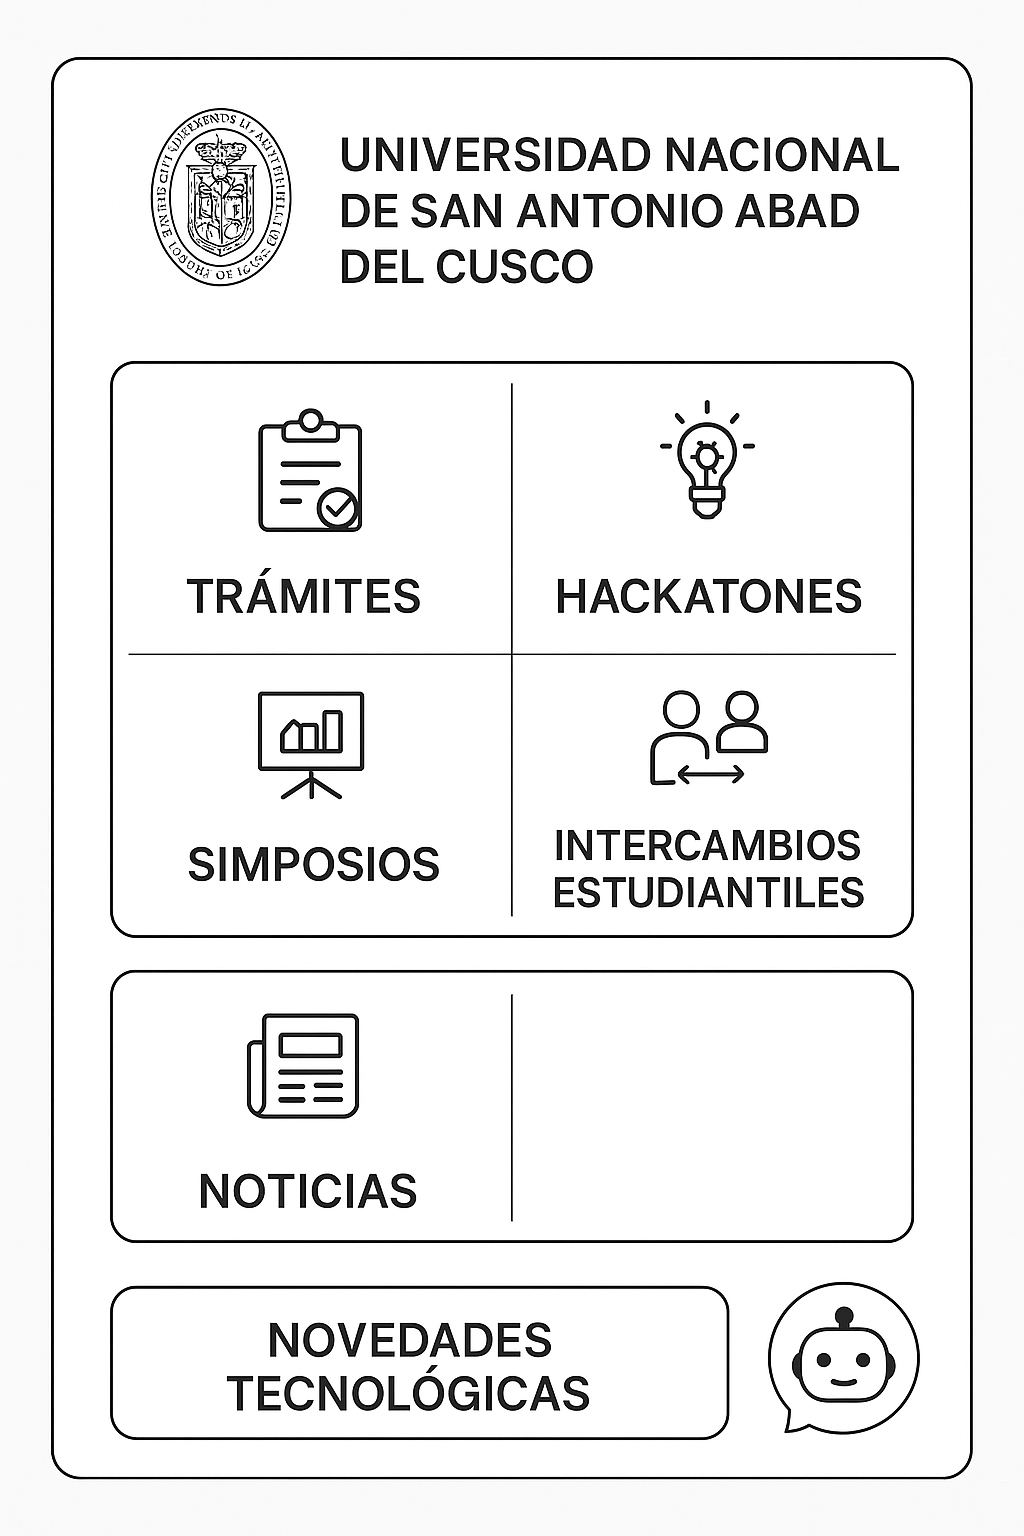
\includegraphics[width=0.47\linewidth,height=12cm,keepaspectratio]{imagenes/concepto_interfaz.png}\par
\captionof{figure}{Diseño conceptual del terminal y de la consulta por categorías}\label{fig:concepto}
\end{center}
Los bocetos orientan la organización visual. La versión funcional se adaptará a las categorías aprobadas, al reproductor y a las pruebas de legibilidad, navegación y accesibilidad.
\begin{center}
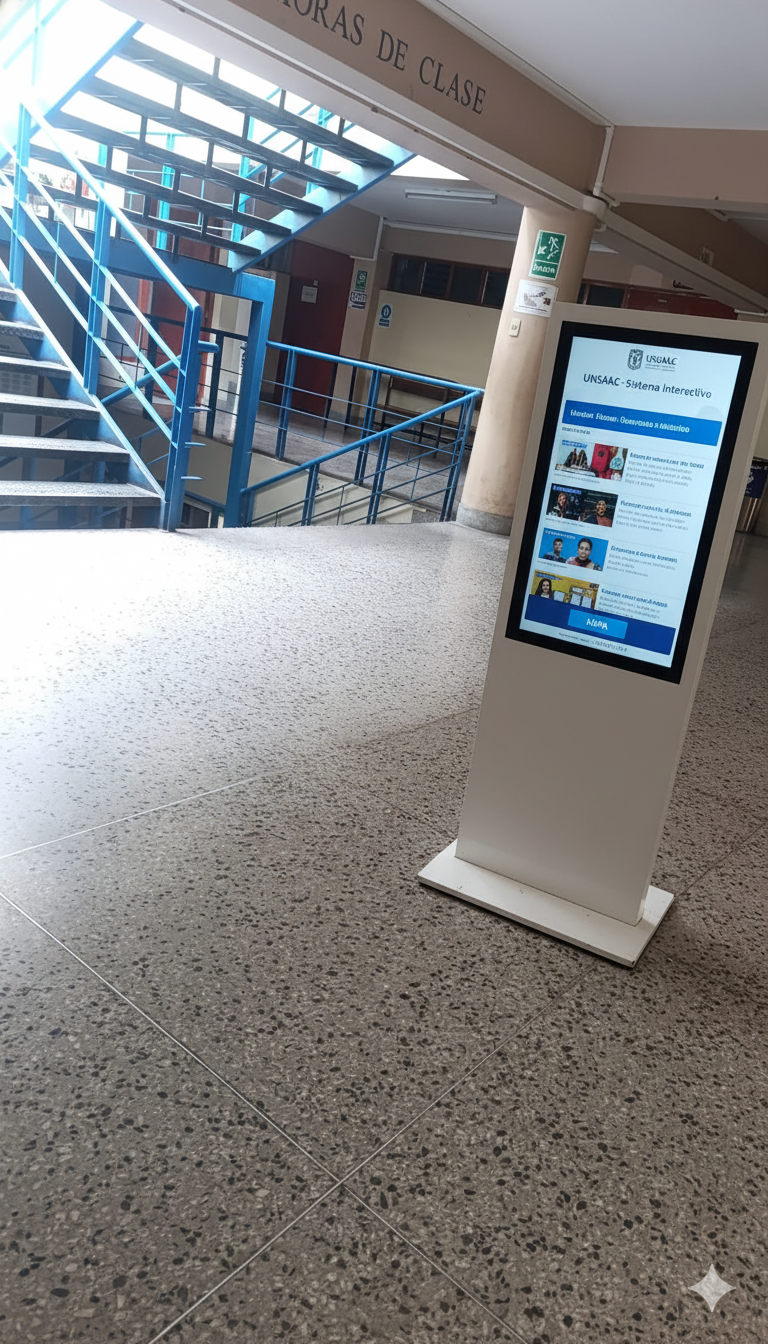
\includegraphics[height=14cm,keepaspectratio]{imagenes/visualizacion_ubicacion.png}\par
\captionof{figure}{Visualización conceptual del emplazamiento propuesto}\label{fig:visualizacion}
\end{center}
\subsection{Datos, interfaces y trazabilidad}
La gestión editorial mantendrá un modelo de información único para las terminales y la consulta móvil. La publicación separará el aviso de sus destinos, de modo que una corrección genere una nueva versión y se propague de forma controlada.

\cuadro{tab:datos}{Modelo lógico de información del servicio}{@{}P{2.5cm}Y Y@{}}{\textbf{Entidad}&\textbf{Datos esenciales}&\textbf{Relación y control}}{
Aviso y versión & Identificador, categoría, título, texto/medio, fuente, emisor y versión & Cada cambio conserva autor y fecha; publicación ligada a una versión\\*
Publicación & Aviso/versión, destino, inicio, vencimiento y aprobación & Un aviso puede publicarse en varios destinos y franjas\\
Terminal & Identificador, piso, cliente, versión aplicada y última comunicación & Destinos por terminal o grupo; estado técnico diferenciado de legibilidad\\
Usuario y permiso & Cuenta, rol, destinos autorizados y estado & Publicación y administración separadas de consulta pública\\
Incidencia & Síntoma, origen, prioridad, responsable y solución & Relacionada con terminal, versión o integración afectada\\
Medición energética & Fecha, intervalo, kWh, origen y calidad del dato & Serie exportable; distingue FV, red, cargas y estimación de batería\\
}
Se documentarán formato de exportación, retención y restauración. Los paquetes de contenido identificarán versión y manifiesto de medios. La recepción comprobará integridad antes de activar una actualización; el cliente conservará una versión funcional de recuperación.

\cuadro{tab:no_funcionales}{Condiciones no funcionales de diseño y prueba}{@{}P{2.6cm}Y@{}}{\textbf{Aspecto}&\textbf{Criterio de trabajo}}{
Respuesta de consulta & Detalle local en hasta 3 s para 95\% de intentos del ensayo; medir con el paquete y equipo previstos\\*
Capacidad inicial & 3 destinos físicos, 500 avisos de prueba y medios con tamaño y formato limitados por política\\
Publicación & Versión aprobada disponible en hasta 5 min en terminal conectada durante el ensayo\\
Disponibilidad & Objetivo inicial 98\% del horario de servicio, con interrupciones y mantenimiento registrados\\
Recuperación & RPO de hasta 24 h para contenido respaldado y RTO de hasta 8 h de atención; restauración ensayada\\
Seguridad y acceso & Administración autenticada, permisos por destino, tráfico protegido y salida del kiosco restringida\\
Mantenibilidad & Inventario, configuración versionada, registros exportables, actualización probada y ruta de sustitución del cliente\\
}
Los objetivos se medirán durante el piloto. La aceptación inicial utilizará los casos de prueba; el seguimiento verificará su continuidad en el horario real de operación.

\subsection{Requerimientos de software y selección de plataforma}
Se compararán dos rutas sobre los mismos casos de uso: \textbf{configurar un CMS de señalización existente} y \textbf{desarrollar un CMS con cliente específico}. La primera puede reducir trabajo inicial; la segunda permite adaptar flujos, pero aumenta responsabilidad de mantenimiento y pruebas.

Xibo ofrece funciones documentadas de usuarios, grupos, pantallas, programación y acciones táctiles \cite{xibousers,xibotouch,xibodisplays}. Permite evaluar un CMS configurable. La compatibilidad del reproductor, las licencias por plataforma y el alojamiento se comprobarán para el conjunto concreto; software abierto no significa implantación ni operación sin costo \cite{xibolic}.

Un cliente web o PWA es otra opción; sus funciones de almacenamiento deben diseñarse y comprobarse. Microsoft documenta que el modo de señalización de Edge utiliza InPrivate \cite{edge}. Por ello, no se garantiza persistencia de contenidos después de reiniciar sólo por utilizar un navegador. El ensayo exigirá reinicio sin red; si la configuración no conserva los paquetes, se requerirá un reproductor con almacenamiento persistente o un paquete local controlado.

\cuadro{tab:software}{Comparación de rutas de software}{@{}P{3.0cm}Y Y@{}}{\textbf{Criterio}&\textbf{CMS configurable}&\textbf{CMS y cliente propios}}{
Publicación y destinos & Configurar funciones existentes y demostrar permisos & Implementar y probar flujo completo\\*
Interacción & Validar acciones táctiles en reproductor real & Diseñar interfaz y navegación específicas\\
Sin conexión & Probar medios descargados y caducidad; URL externa no queda copiada automáticamente & Diseñar caché persistente, versiones y recuperación\\
Costo & Configuración, licencias aplicables, alojamiento y soporte & Análisis, desarrollo, pruebas, despliegue y mantenimiento\\
Decisión & Preferible si satisface los casos sin extensiones costosas & Justificable si hay brechas funcionales relevantes y capacidad de soporte\\
}
Se recomienda demostrar primero la ruta configurable. El presupuesto reserva trabajo de adaptación; si los ensayos exigen desarrollo mayor, se revisará esfuerzo y alternativa antes de comprometer alcance.

\subsection{Hardware y ubicación}
\cuadro{tab:hardware}{Especificaciones funcionales del piloto}{@{}P{3.0cm}Y P{2.5cm}@{}}{\textbf{Componente}&\textbf{Características propuestas}&\textbf{Cantidad}}{
Terminal completo & Interior, piso anclable, aproximadamente 55 pulgadas, vertical 4K, mínimo 10 contactos táctiles y acceso técnico protegido & 3 unidades\\*
Visualización & Panel 4K vertical; brillo de referencia mínimo 400 nits en interior y legibilidad verificada; 450 a 500 nits preferibles con reflejos & En cada terminal\\
Cómputo y sistema & Cliente Windows con 16 GB/256 GB como referencia, o Android con recursos demostrados; sistema licenciado y soporte documentado & Integrado o incluido\\
Red & Cableado Cat 6 de cobre, switch administrable y gabinete; direccionamiento y segmentación acordados; Wi-Fi sólo si se valida & 7 enlaces y 1 gabinete\\
Videovigilancia & Una cámara IP por terminal y grabador local con 30 días de conservación & 3 cámaras y 1 NVR\\
CMS y respaldo & Alojamiento, copias separadas, cuentas de gestión y recuperación & 1 servicio central\\
Alimentación & Circuito de cargas críticas, protecciones y puesta a tierra según diseño; FV y batería compatibles & 1 sistema integrado\\
}
El cuadro resume la función de cada componente. Los mínimos exigibles, sin marca ni modelo, se desarrollan como especificaciones ET-01 a ET-10 en la sección \ref{sec:especificaciones}. La opción de mercado usada para valorizar cada uno se elige en la sección \ref{sec:seleccion}. El suministro identificará CPU exacta, edición y licencia del sistema, potencia máxima, garantía e instalación.

Se adopta una cota de diseño de 200 W por terminal completo. Las ofertas comparadas publican 95 W sin condición de medición, y la ficha de una ruta Android de 55 pulgadas declara 108 W típicos y 155 W máximos \cite{prodimer,hikvision}. Una oferta con mayor consumo obligará a recalcular el sistema energético. El horario del servicio es de 12 horas al día. La aprobación de un cliente Android incluirá instalación del reproductor, persistencia, legibilidad y soporte de actualizaciones.

La distribución por piso y la propuesta de interfaz se desarrollan en las secciones siguientes. El diseño de instalación incluirá circulación, alcance de uso, anclajes y condiciones de mantenimiento.

\subsection{Emplazamiento y distribución del piloto}
Se plantea un terminal por piso. El levantamiento contrastará las posiciones de los planos con tránsito, visibilidad, reflejos, aproximación, circulación y acceso de mantenimiento. La definición final incorporará los recorridos de red y del circuito protegido.

\subsubsection{Primer piso}
\begin{center}
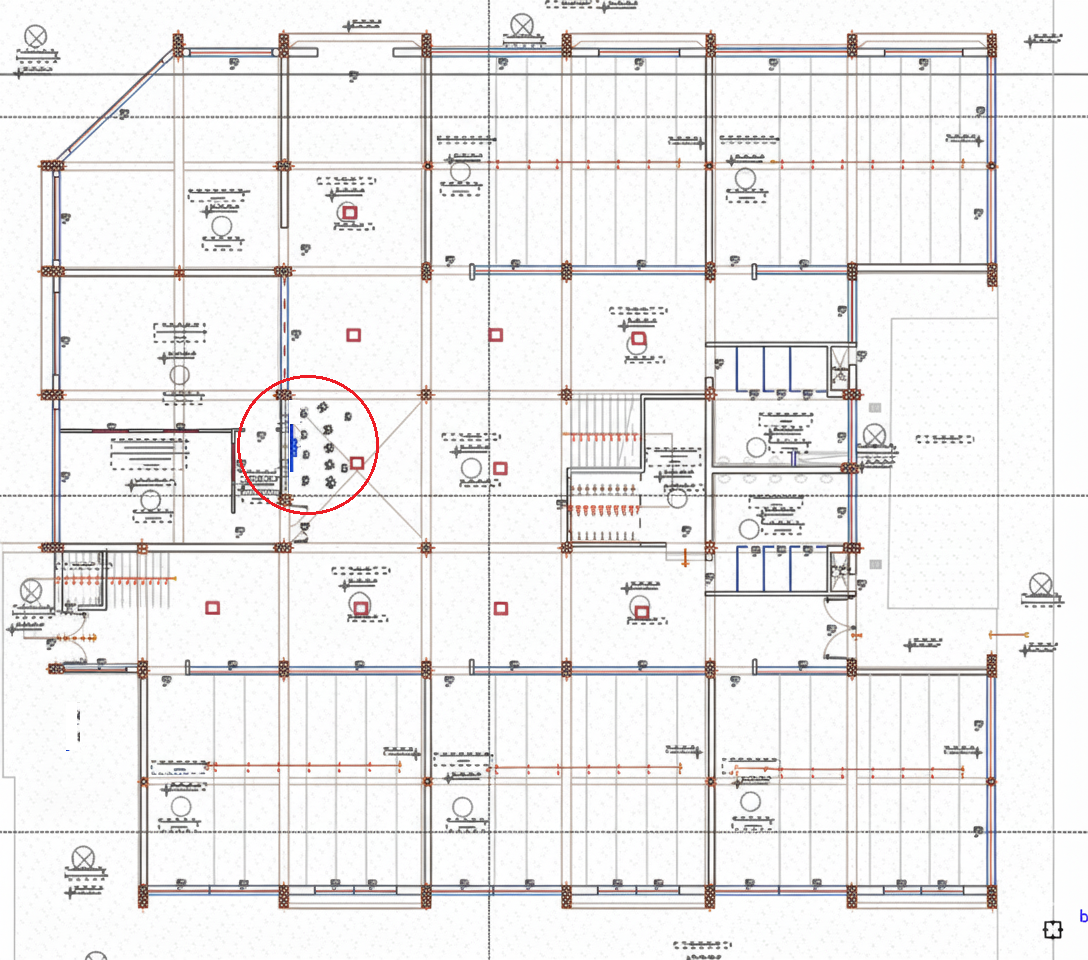
\includegraphics[width=\linewidth,height=12.2cm,keepaspectratio]{imagenes/planta_piso_1.png}\par
\vspace{0.15cm}
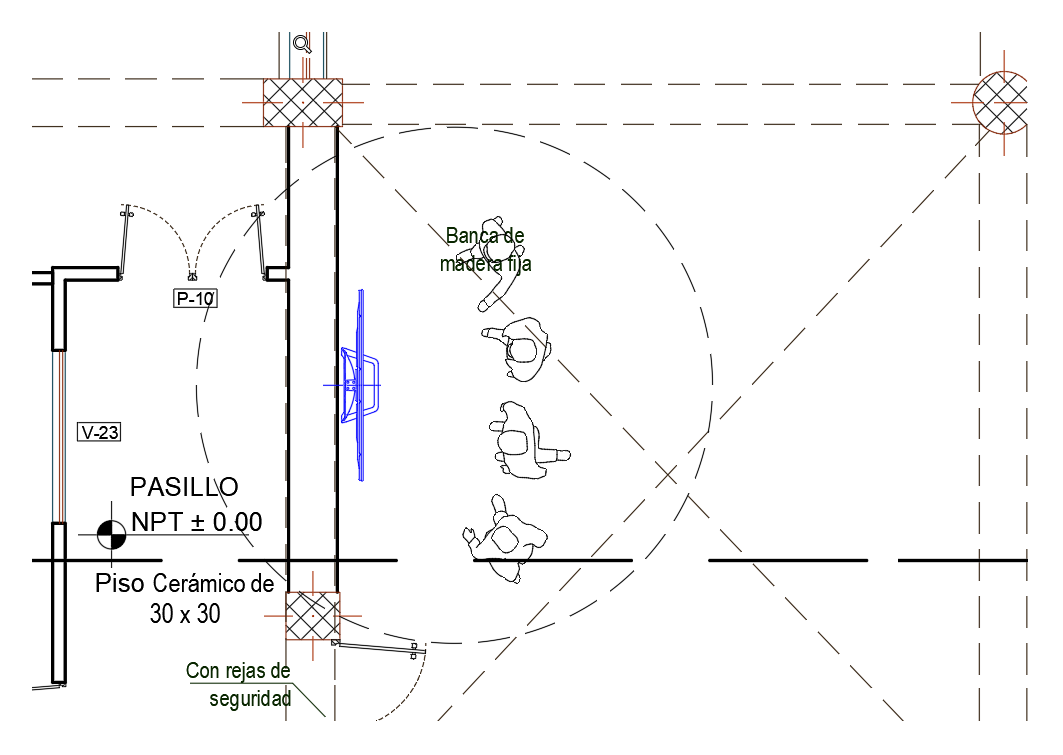
\includegraphics[width=\linewidth,height=5.0cm,keepaspectratio]{imagenes/detalle_piso_1.png}\par
\captionof{figure}{Planta y detalle de ubicación propuesta en el primer piso}\label{fig:piso1}
\end{center}
\clearpage
\subsubsection{Segundo piso}
\begin{center}
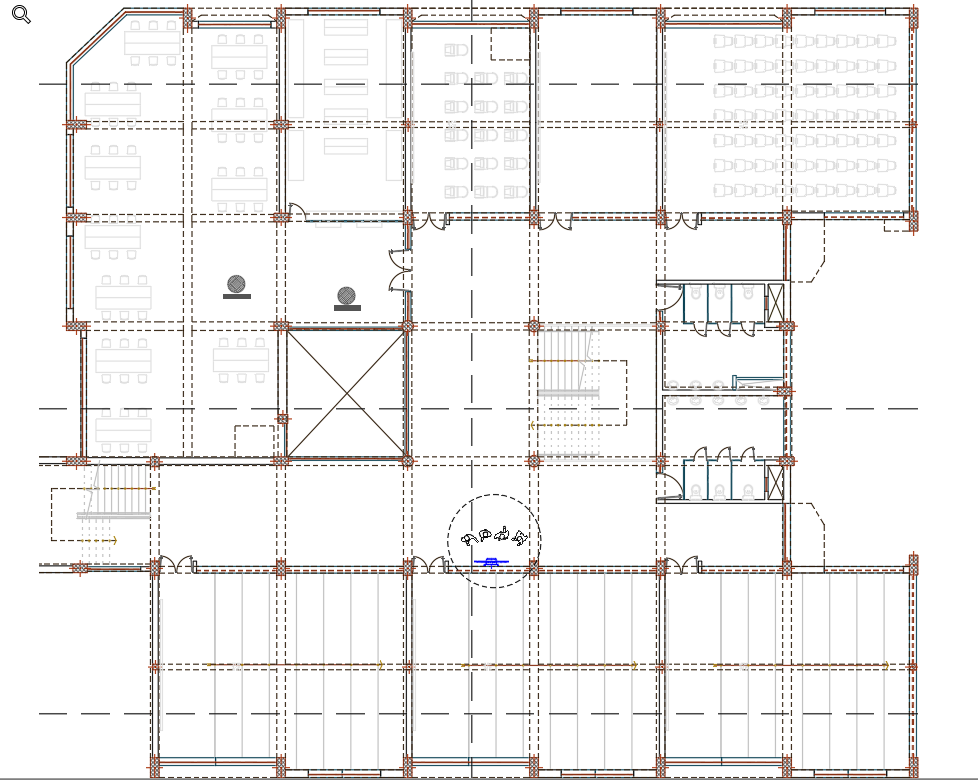
\includegraphics[width=\linewidth,height=13cm,keepaspectratio]{imagenes/planta_piso_2.png}\par
\vspace{0.25cm}
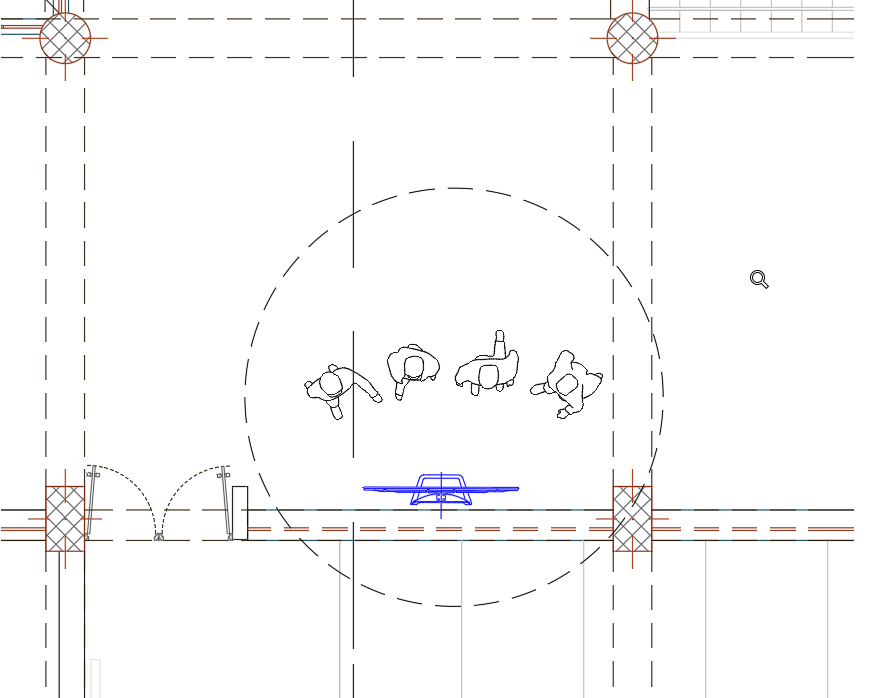
\includegraphics[width=\linewidth,height=5.5cm,keepaspectratio]{imagenes/detalle_piso_2.png}\par
\captionof{figure}{Planta y detalle de ubicación propuesta en el segundo piso}\label{fig:piso2}
\end{center}
\clearpage
\subsubsection{Tercer piso}
\begin{center}
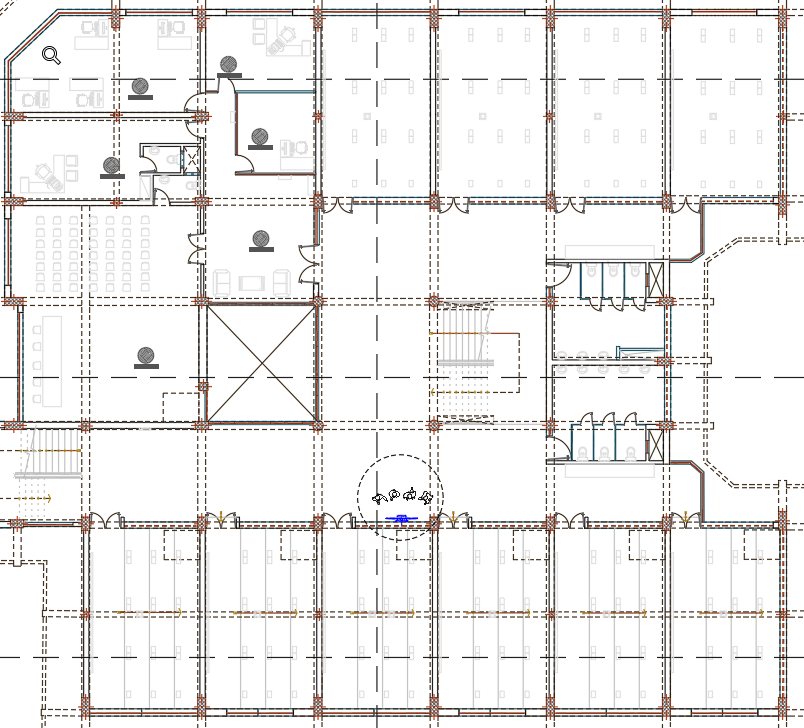
\includegraphics[width=\linewidth,height=13cm,keepaspectratio]{imagenes/planta_piso_3.png}\par
\vspace{0.25cm}
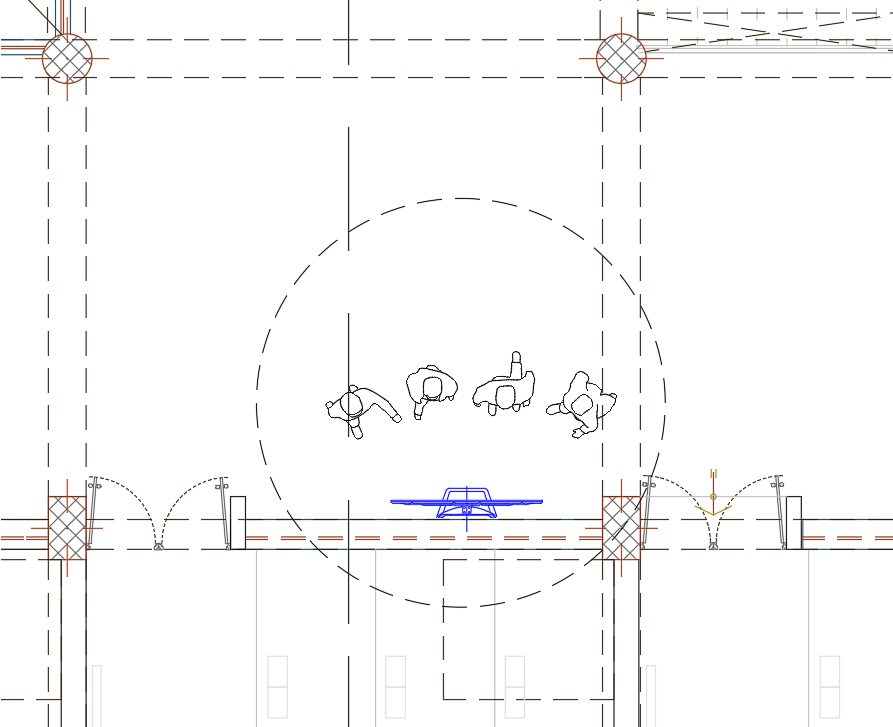
\includegraphics[width=\linewidth,height=5.5cm,keepaspectratio]{imagenes/detalle_piso_3.png}\par
\captionof{figure}{Planta y detalle de ubicación propuesta en el tercer piso}\label{fig:piso3}
\end{center}
\clearpage

\subsection{Seguridad, accesibilidad y continuidad}
\begin{itemize}
\item Cuentas individuales para administración; permisos por función y destino; consulta pública sin acceso al escritorio ni a la edición.
\item Conexión protegida, actualizaciones controladas, dominios autorizados y credenciales fuera de la interfaz pública.
\item Botones legibles, contraste, retorno al inicio por inactividad y alternativa mediante QR; altura y aproximación verificadas en la ubicación.
\item Audio desactivado por defecto o limitado según condiciones del espacio. No depender sólo de audio o color para comunicar información.
\item Copia diaria inicial de CMS, medios y configuración; ensayo de restauración. Objetivos de trabajo: pérdida de datos recuperables hasta 24 h y recuperación en 8 h de atención, por acordar con TI.
\item Durante desconexión, mostrar última sincronización y consultar sólo contenido local permitido por su vigencia. Las alertas urgentes no se presentarán como actuales sin confirmación.
\end{itemize}
La última comunicación del cliente no demuestra por sí sola que la pantalla esté encendida o sea legible. Se combinará supervisión técnica con comprobación visual y reporte de usuarios.

\subsection{Comparación tecnológica de módulos fotovoltaicos}
Se contrastan cuatro módulos publicados por un mismo distribuidor en Perú, AutoSolar, para homogeneizar IGV, existencias y despacho. La selección considera costo por Wp, corriente frente al límite de 16~A del seguidor MPPT, tensión del string en frío, área, masa y garantía, además de la potencia nominal. Cuando la página comercial y la ficha del fabricante difieren, prevalece la ficha. Una generación tecnológica más reciente puede mejorar el aprovechamiento del área, pero no demuestra por sí sola menor costo del servicio ni compatibilidad con el inversor. El cuadro \ref{tab:modulos_comparados} presenta las cuatro opciones con su imagen referencial, datos de ficha, precio y enlaces.

Jinko conserva el menor costo por Wp y se mantiene como referencia de valorización. Su Imp STC deja un margen de 5,3\% frente a los 16~A del seguidor, pero la corriente bifacial BNPI de 16,73~A lo supera: no se presupone ganancia posterior y se evaluará la limitación de corriente \cite{jinko}. AutoSolar declara además una garantía propia de un año en esa página; la garantía de 12 años corresponde al fabricante y su atención deberá acreditarse \cite{preciojinko}.

La página de Trina anuncia un módulo bifacial, mientras la ficha que enlaza corresponde al TSM-NE19R.70 de lámina posterior \cite{trinaprecio,trinaficha}. La oferta deberá identificar el modelo exacto. Si se confirma esa ficha, el conjunto pesa 28,2~kg menos y amplía el margen de corriente por S/~168,30 adicionales. LONGi Hi-MO X10 ofrece la mayor eficiencia y 15 años de garantía de producto, con S/~926,04 adicionales y el menor margen de corriente. El módulo LONGi de 505~W es la única opción con holgura amplia frente al seguidor; utiliza tecnología PERC, requiere siete unidades y eleva el costo en S/~2\,355,90 \cite{longi505ficha}.

\textbf{Opción elegida para valorizar ET-06: Jinko Tiger Neo de 615~W}, por menor costo por Wp entre las que cumplen tensión, área y garantía. Las cuatro tensiones del string en frío permanecen bajo los 550~V del inversor elegido y dentro de su rango MPPT de 40 a 530~V. Si la ingeniería concluye que la limitación de corriente del módulo de referencia es inaceptable, se confirmará el Trina de lámina posterior, se adoptará el módulo de 505~W o se cotizará un inversor con mayor corriente por seguidor; cualquiera de esas decisiones requerirá recalcular el conjunto. Las garantías de ficha no reemplazan las condiciones contractuales, exclusiones y atención local que debe acreditar el proveedor.

\begin{table}[p]\formatofichas
\caption{Paneles solares analizados como opción: características STC y precio unitario}\label{tab:modulos_comparados}
\begin{tabularx}{\linewidth}{@{}>{\raggedright\arraybackslash}p{2.15cm}YYYY@{}}
\toprule
\textbf{Característica} & \textbf{Jinko Tiger Neo 615~W} & \textbf{Trina Vertex N 625~W} & \textbf{LONGi Hi-MO X10 640~W} & \textbf{LONGi Hi-MO 5 505~W}\\\midrule
\textbf{Imagen referencial} & \imgficha{imagenes/mercado_fv_jinko615.jpg}{3.1cm} & \imgficha{imagenes/mercado_fv_trina625.jpg}{3.1cm} & \imgficha{imagenes/mercado_fv_longi640.jpg}{3.1cm} & \imgficha{imagenes/mercado_fv_longi505.jpg}{3.1cm}\\
\textbf{Modelo y tecnología} & JKM615N-66HL4M-BDV; TOPCon tipo N, bifacial, doble vidrio & TSM-NE19R.70 según la ficha: i-TOPCon con lámina posterior; la página dice bifacial & LR8-66HVD-640M; contacto posterior HPBC 2.0, bifacial, doble vidrio & LR5-66HPH-505M; PERC de media celda, vidrio simple; ficha de 2022\\
\textbf{Potencia y eficiencia} & 615 Wp; 22,77\% & 625 Wp; 23,1\% & 640 Wp; 23,7\% & 505 Wp; 21,3\%\\
\textbf{Vmp / Imp STC} & 40,60 V / 15,15 A & 41,6 V / 15,00 A & 40,78 V / 15,69 A & 38,53 V / 13,11 A\\
\textbf{Voc / Isc STC} & 48,88 V / 16,02 A & 49,8 V / 15,93 A & 49,52 V / 16,38 A & 45,70 V / 13,97 A\\
\textbf{Coeficiente de Voc} & $-0{,}25$\,\%/°C & $-0{,}24$\,\%/°C & $-0{,}20$\,\%/°C & $-0{,}265$\,\%/°C\\
\textbf{Medidas y masa} & 2\,382 $\times$ 1\,134 $\times$ 30 mm; 32,4 kg & 2\,382 $\times$ 1\,134 $\times$ 30 mm; 27,7 kg & 2\,382 $\times$ 1\,134 $\times$ 30 mm; 33,5 kg & 2\,093 $\times$ 1\,134 $\times$ 35 mm; 25,3 kg\\
\textbf{Garantía} & 12 y 30 años & 12 y 25 años & 15 y 30 años & 12 y 25 años\\
\textbf{Precio con IGV} & S/~405,35; S/~0,659 por Wp; sin IGV S/~343,52 & S/~433,40; S/~0,693 por Wp; sin IGV S/~367,29 & S/~559,69; S/~0,875 por Wp; sin IGV S/~474,31 & S/~684,00; S/~1,354 por Wp; sin IGV S/~579,66\\
\textbf{Conjunto para el balance} & 6 módulos; 3,69 kWp; S/~2\,432,10; 16,21 m$^2$; 194,4 kg & 6 módulos; 3,75 kWp; S/~2\,600,40; 16,21 m$^2$; 166,2 kg & 6 módulos; 3,84 kWp; S/~3\,358,14; 16,21 m$^2$; 201,0 kg & 7 módulos; 3,535 kWp; S/~4\,788,00; 16,61 m$^2$; 177,1 kg\\
\textbf{Margen de Imp a 16 A} & 5,3\%; la corriente BNPI de 16,73 A lo supera & 6,3\%; sin ganancia posterior si se confirma la ficha & 1,9\%; con 5\% de ganancia posterior, unos 16,47 A; la ficha tabula 16,57 A sobre base de 645 W & 18,1\%; módulo monofacial\\
\textbf{Voc del string a $-10$\,°C} & 318,94 V & 323,90 V & 317,92 V & 349,57 V\\
\textbf{Enlace del producto} & \enlace{https://autosolar.pe/paneles-solares-24v/panel-solar-jinko-tiger-neo-bifacial-615w-n-type} & \enlace{https://autosolar.pe/paneles-solares/panel-solar-bifacial-625w-trina-solar} & \enlace{https://autosolar.pe/paneles-solares-24v/panel-solar-bifacial-longi-lr8-66hvd-640m-hi-mo-640w} & \enlace{https://autosolar.pe/paneles-solares-24v/panel-solar-longi-lr5-66hph-himo5-505w}\\
\bottomrule
\end{tabularx}
\fuentefichas{Páginas de AutoSolar Perú y fichas de fabricante consultadas el 30 de octubre de 2026 \cite{preciojinko,jinko,trinaprecio,trinaficha,longiprecio2026,longificha2025,longi505precio,longi505ficha}. STC corresponde a condiciones normalizadas de ensayo; la garantía indica años de producto y de potencia lineal. El número de módulos es $N=\lceil 1{,}20(8{,}16)/(3P)\rceil$, con $P$ en kW, 4 HSP y factor 0,75; el margen de corriente es $(16-I_{mp})/16$. Fuente de las imágenes, de izquierda a derecha: \url{https://cdn.autosolar.pe/images/1002232/panel-solar-jinko-tiger-neo-bifacial-615w-n-type-684992fe19b4e.jpg}; \url{https://cdn.autosolar.pe/images/1002343/panel-solar-bifacial-625w-trina-solar-698dfb53e7a67.jpg}; \url{https://cdn.autosolar.pe/images/1006015/panel-solar-bifacial-longi-lr8-66hvd-640m-hi-mo-640w-69a9f09bd1a5f.jpg}; \url{https://cdn.autosolar.pe/images/1006012/panel-solar-longi-lr5-66hph-himo5-505w.jpg}. Las imágenes son referenciales, se reproducen con fines académicos y su procedencia se registra en \texttt{procedencia\_imagenes.json}.}
\end{table}

\subsection{Conjunto energético de referencia y compatibilidad}
El conjunto valorizado comprende \textbf{seis módulos de 615 Wp, un inversor híbrido monofásico de 4 kW y una batería LFP de 48 V y 4,8 kWh}. Cumplen las especificaciones ET-05 a ET-07 de la sección \ref{sec:especificaciones}. Las opciones de mercado que los valorizan se eligen en los cuadros comparativos de la sección \ref{sec:seleccion}. Quedan sujetos a la condición G1 de aceptación técnica y a la oferta final; una variante equivalente acreditará su propia ficha y compatibilidad.

La ficha del inversor elegido acredita: tensión FV máxima de 550 V, rango MPPT de 40 a 530 V con 380 V nominales y arranque a 50 V; dos seguidores con una cadena cada uno, 16 A de entrada y 20 A de cortocircuito por seguidor; y hasta 6\,500 Wp de generador. También acredita batería de 48 V con rango de 40 a 60 V, 100 A de carga y descarga, salida de respaldo de 5\,000 VA con conmutación de hasta 10 ms, eficiencia máxima de 97,6\%, grado IP66 y comunicación RS485/CAN. Su altitud máxima de operación es de 4\,000 m, con reducción de potencia sobre 3\,000 m \cite{tensiteinv}. Cusco se ubica cerca de 3\,400 m, de modo que la reducción aplica; con 640 W de carga simultánea el margen sigue siendo amplio, pero la oferta precisará la potencia disponible a la cota real. Estos límites no equivalen a aprobar una cadena sólo por su potencia total.

% Flotante para que conserve el orden después del cuadro comparativo de módulos.
\begin{table}[htbp]
\cuadro{tab:string_referencia}{Comprobación preliminar de seis módulos de referencia en serie}{@{}Y P{4.7cm}@{}}{\textbf{Magnitud}&\textbf{Resultado ilustrativo}}{
Potencia; tensión de máxima potencia STC & 3\,690 Wp; $6(40,60)=243,60$ V\\*
Tensión de circuito abierto STC & $6(48,88)=293,28$ V\\
Corrientes STC del string & Imp 15,15 A; Isc 16,02 A\\
Voc con temperatura supuesta de $-10\,^{\circ}$C & $293,28[1+(-0,0025)(-10-25)]=318,94$ V\\
Comparación con el inversor elegido & 318,94 V $<$ 550 V; 243,60 V dentro de 40 a 530 V; 16,02 A $<$ 20 A\\
}
\end{table}
El cuadro \ref{tab:string_referencia} resume la comprobación de la cadena. Su cálculo de Voc utiliza el coeficiente de $-0,25\%/^{\circ}$C y una temperatura de ensayo supuesta; no es un registro del edificio ni un diseño ejecutivo. Se comprobarán temperatura mínima, tolerancias, tensión MPPT en caliente, orientación y sombras. La corriente permanece igual en serie. Dividir tres módulos por seguidor reduce el margen de tensión y requiere otra comprobación; dos strings en paralelo sobre un mismo seguidor sumarían Isc de 32,04 A STC, superior a 20 A.

La ficha del módulo declara Imp de 16,73 A e Isc de 17,70 A en condiciones bifaciales BNPI \cite{jinko}. La primera supera los 16 A del MPPT y puede producir limitación de corriente y energía. Se requiere evaluación de fabricante o instalador, separando corriente operativa y de cortocircuito con sus correcciones; no se presupone ganancia bifacial.

La batería elegida es del mismo fabricante que el inversor, lo que facilita la compatibilidad del BMS por CAN/RS485; la oferta confirmará protocolo, firmware y configuración. Su ficha acredita química LiFePO4, 4,8 kWh de energía total y 4,3 kWh utilizables, 60 A nominales y 100 A continuos de descarga. Indica además más de 6\,000 ciclos al 80\% de profundidad, carga entre 0 y 50\,°C, descarga entre $-10$ y 55\,°C, uso interior con IP20, 43 kg, garantía de cinco años y certificaciones UN38.3, CE y TÜV \cite{tensitebat}. La ficha no publica altitud: la oferta la acreditará para la cota de Cusco. La garantía de cinco años coincide con la reposición prevista en el año 5 del flujo económico.

\subsection{Integración, materiales y condición de habilitación}
Se plantea una operación híbrida con respaldo de red y \textbf{consigna programada de exportación cero}, con un medidor bidireccional Modbus compatible con el inversor y un módulo de monitoreo con registro exportable (ET-10) \cite{autosolarmed}. El control depende del muestreo y admite sobreimpulsos transitorios, por lo que la consigna no demuestra aislamiento físico ni ausencia instantánea de exportación. La ingeniería definirá el punto de conexión, neutro, tierra, protecciones y las condiciones institucionales aplicables. Si exige impedir físicamente la realimentación, incorporará una solución específica aprobada, sin atribuir esa función al simple ajuste del inversor.

\cuadro{tab:bom_energia}{Cantidades del subsistema energético para cotizar e integrar}{@{}P{3.4cm}P{1.8cm}Y@{}}{\textbf{Elemento}&\textbf{Cantidad}&\textbf{Condición de suministro e ingeniería}}{
Módulos FV, ET-06 & 6 & Modelo, conectores, estructura y distribución verificados\\*
Inversor híbrido, ET-05 & 1 & Corriente por MPPT, altitud y compatibilidad BMS acreditadas\\
Batería LFP, ET-07 & 1 & Protocolo, cable BMS, fusible y soporte confirmados\\
Medidor y monitoreo, ET-10 & 1 y 1 & Comunicación Modbus y registro exportable verificados\\
Estructura, ET-08 & 2 de 3 módulos & Compatibilidad con 2\,382 × 1\,134 mm y anclaje a la cubierta\\
Protección DC, ET-09 & 1 conjunto & Interruptor DC de 25 A, protector de sobretensiones y 30 m de cable de 6 mm² por polaridad\\
Tablero crítico, ET-09 & 1 & 18 polos: entrada y salida 2P 32 A, dos circuitos 2P 16 A con diferencial y protector AC\\
Puesta a tierra, ET-09 & 1 pozo & Barra de cobre de 2,4 m, cemento conductivo y medición de resistencia\\
}
Los precios de estos elementos proceden de publicaciones identificadas y se detallan en el cuadro \ref{tab:precios_energia}. Las cantidades de conductores AC y canalización son estimaciones de metrado. El monitoreo y los enlaces RS485 del medidor y CAN del BMS deberán ser compatibles, con pinout y accesorios confirmados. Se evitará cotizar dos veces medidor, cables o soportes incluidos en los equipos.

La condición \textbf{G1, previa a compra y montaje}, requiere ficha y oferta del modelo y revisión, altitud real, balance de cargas, configuración del string con frío, calor y corriente bifacial, compatibilidad BMS y firmware, esquema unifilar y autorización de conexión que corresponda. La ingeniería fijará longitudes, secciones, caída de tensión, canalizaciones, seccionamiento y protección DC, AC y de batería, sobretensiones, diferencial adecuado, puesta a tierra, anclajes y capacidad de cubierta. La aceptación incluirá registros exportables de energía y eventos, pérdida de comunicación, transferencia y ensayo de respaldo con la carga acordada.

\subsection{Sistema de alimentación fotovoltaica}
La topología propuesta suministrará un circuito de cargas críticas mediante generación FV, banco de batería e inversor/cargador con respaldo de red y aislamiento apropiado. Se propone operación sin exportación programada, con medidor compatible, CT y consignas verificadas. El diseño definirá la conexión de red, el circuito de respaldo, la transferencia, el tratamiento de neutro y tierra y las protecciones de interconexión. El control de exportación limita flujos mediante medición; el aislamiento y la prevención de realimentación se comprobarán mediante el esquema eléctrico y sus pruebas.

\begin{center}
\begin{tikzpicture}[>=Latex,node distance=9mm,every node/.style={font=\small,align=center},box/.style={draw,text width=4.0cm,minimum height=1.0cm,inner sep=5pt}]
\node[box] (pv) {Módulos FV\\Seccionamiento y protección DC};
\node[box,right=17mm of pv] (inv) {Inversor/cargador\\MPPT y gestión de energía};
\node[box,below=of pv] (bat) {Batería con BMS\\Protección y maniobra DC};
\node[box,below=of inv] (red) {Red de respaldo\\Transferencia y aislamiento};
\node[box,below=18mm of bat,text width=10cm] (load) {Circuito protegido de cargas críticas\\Tres terminales, switch, NVR y cámaras};
\draw[->](pv)--(inv);\draw[<->](bat.east)--(inv.south west);
\draw[->](red)--(inv);\draw[->](inv.east)--++(8mm,0)|-(load.east);
\end{tikzpicture}
\captionof{figure}{Esquema funcional de alimentación; unifilar por desarrollar}
\label{fig:energia}
\end{center}
La solución central de respaldo se comprobará con las fuentes de alimentación de los terminales y el tiempo de transferencia. Cualquier UPS local adicional tendrá una función específica y se incorporará al presupuesto después del ensayo.

\subsection{Recurso solar de referencia}
Se consultó NASA POWER para el punto regional aproximado $13,52^\circ$ S y $71,96^\circ$ O, utilizando las medias mensuales de 2021 a 2025 \cite{nasa}. La irradiación horizontal media anual del conjunto es 4,83 kWh/m$^2$/día; los promedios mensuales de los cinco años varían de 4,48 a 5,27. La menor media mensual individual de la serie es 4,10. Se adopta 4 HSP para el escenario de diseño y 3 HSP para sensibilidad.
\begin{center}
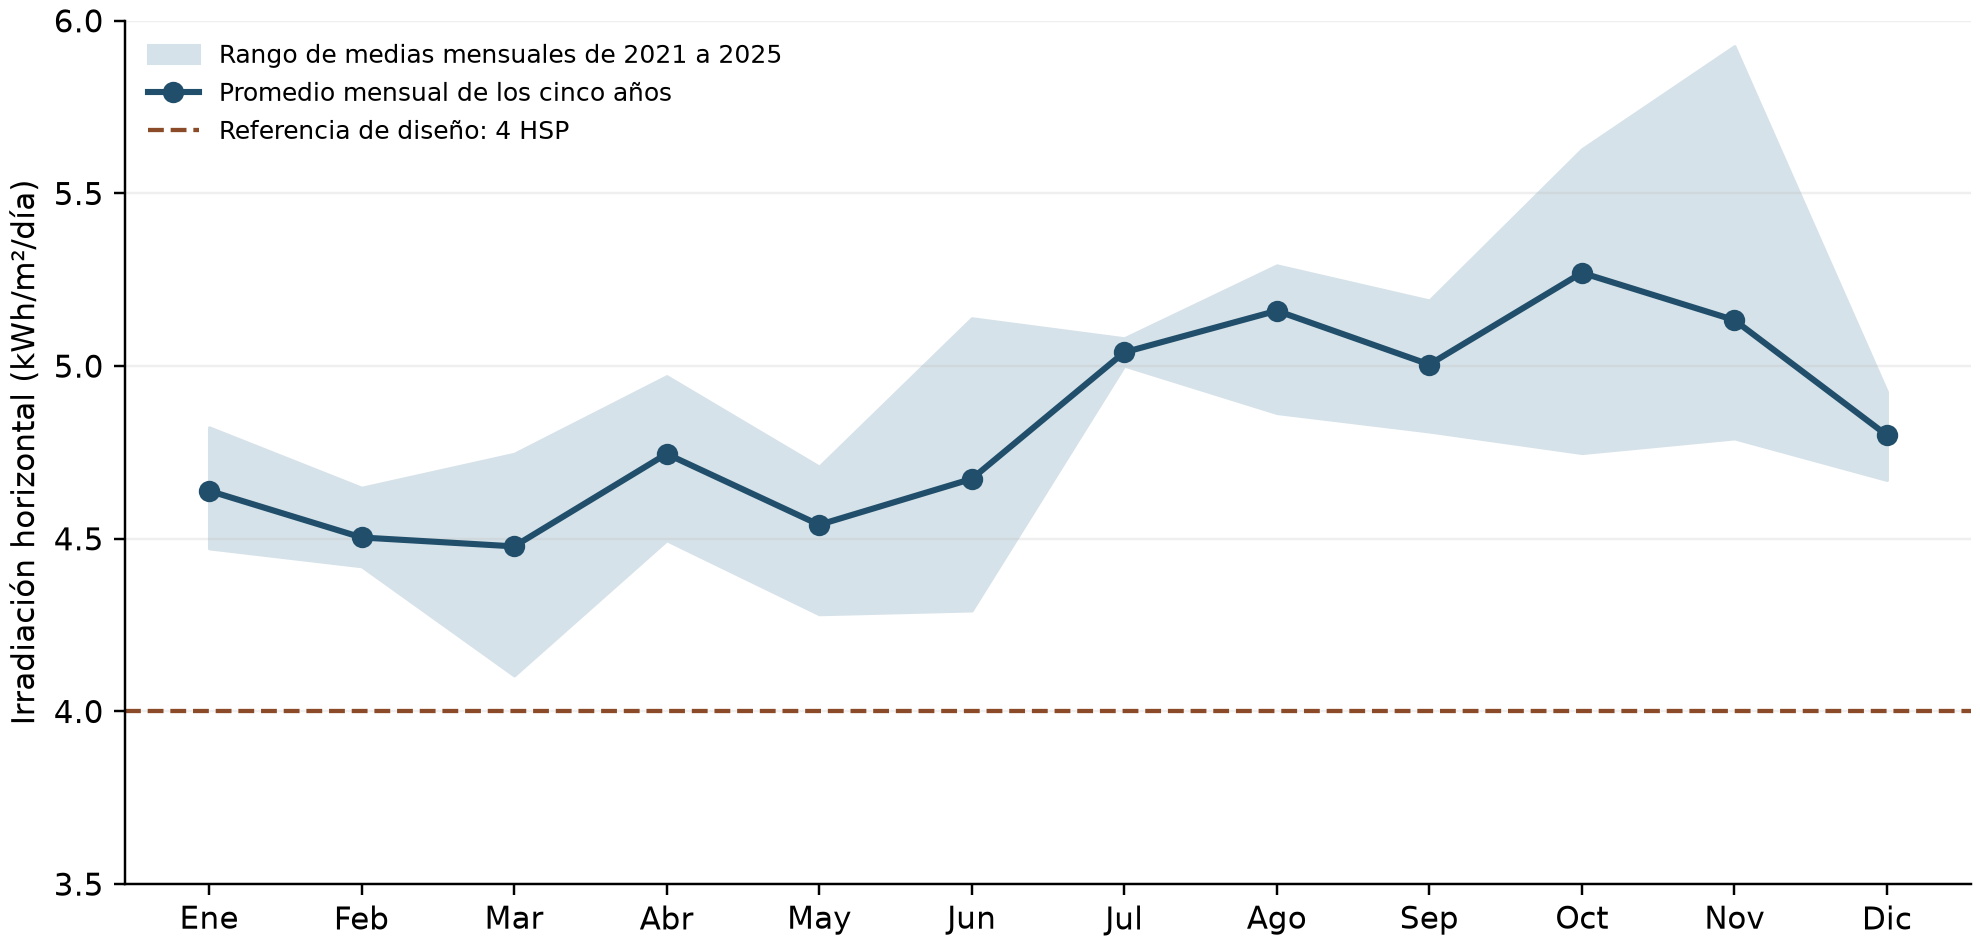
\includegraphics[width=\linewidth]{imagenes/recurso_solar_nasa.png}\par
\captionof{figure}{Recurso solar regional de referencia, NASA POWER 2021 a 2025}\label{fig:recurso}
\end{center}
La serie es un producto regional, no una medición de cubierta. La ingeniería incorporará coordenadas y cota del sitio, orientación, inclinación, sombras e irradiación sobre el plano de módulos. La aproximación horizontal se utiliza para el balance de formulación; las medias mensuales no describen cada día de nubosidad.
\subsection{Balance energético de formulación}
El cuadro \ref{tab:energia} fija supuestos de cálculo. La potencia del terminal completo deberá reemplazarse por ficha o medición con el brillo, cliente y periféricos reales.

\cuadro{tab:energia}{Supuestos y resultados del escenario energético}{@{}Y P{4.5cm}@{}}{\textbf{Variable}&\textbf{Valor de formulación}}{
Terminales y consumo completo supuesto & 3 unidades de 200 W cada una\\*
Horario activo; apagado fuera de servicio & 12 h/día; 0 W restante supuesto\\
Comunicaciones y videovigilancia & 40 W, 24 h/día; desglose en el cuadro \ref{tab:cargas}\\
Potencia simultánea & $3(200)+40=640$ W\\
Energía diaria de cargas & $3(0,200)(12)+0,040(24)=8,16$ kWh/día\\
Energía para 4 horas de corte & $0,640(4)=2,56$ kWh AC\\
Generación propuesta para estudiar & $6(615)=3\,690$ Wp, es decir 3,69 kWp\\
Recurso y factor global supuestos & 4 HSP/día; factor 0,75\\
Producción ilustrativa & $3,69(4)(0,75)=11,07$ kWh/día\\
Sensibilidad con 3 HSP & 8,3025 kWh/día, antes de revisar auxiliares\\
}
HSP significa horas solares pico equivalentes. Los 4 HSP son una referencia conservadora respecto de las medias mensuales regionales; el factor 0,75 es un supuesto global de conversión. El diseño incorporará el plano de captación, las sombras y el periodo crítico. No se computa ganancia bifacial sin geometría y albedo comprobados, ni se añaden dos veces pérdidas ya incluidas en el factor.

El mínimo aritmético con margen de 20\% sería:
\[
N_{\mathrm{FV}}=\left\lceil\frac{1,20(8,16)}{0,615(4)(0,75)}\right\rceil=6.
\]
Si se incorpora como sensibilidad un consumo propio adicional de 15 W del inversor durante 24 h, la carga equivalente aumenta a 8,52 kWh/día. Ese consumo es también supuesto; se reemplazará por dato del equipo y se delimitarán las pérdidas. Con 3 HSP, los 8,3025 kWh/día no cubrirían dicho escenario: se demuestra la dependencia del recurso y del horario.

Para una batería nominal de 4,8 kWh, una profundidad de descarga de diseño de 80\%, capacidad remanente de 80\% y rendimiento batería a salida AC de 90\% permiten comprobar:
\[
E_{\mathrm{AC,diseño}}=4,8(0,80)(0,80)(0,90)=2,7648\ \mathrm{kWh}.
\]
El resultado supera 2,56 kWh con una holgura limitada; se deben descontar auxiliares y efectos de temperatura. No equivale a una garantía de cuatro horas. La capacidad de energía se relacionará con la tensión y los Ah de la referencia exacta.

\subsection{Condiciones del emplazamiento y del montaje}
La ingeniería contrastará cubierta, sombras, acceso, carga, anclajes e impermeabilización. La superficie geométrica de los seis módulos de referencia es 16,21 m$^2$ y su masa es 194,4 kg; el diseño añadirá estructura, separaciones y condiciones de trabajo seguro.

Se definirán estructura y tornillería, inclinación y orientación, conductores por corriente y recorrido, conectores compatibles y canalizaciones. El suministro incluirá seccionamiento, protección próxima a batería, sobrecorriente, sobretensiones, protección diferencial indicada, tierra, equipotencialidad y señalización según el diseño.

La instalación entregará unifilar, ajustes, metrado, registros de pruebas, manual y responsable de mantenimiento. Los siete enlaces de red y los recorridos del circuito crítico se conciliarán con las plantas y la accesibilidad del terminal; su metrado de partida figura en la sección \ref{sec:especificaciones}.

\subsection{Escalabilidad y flexibilidad}
El CMS identificará terminal, grupo y versión del paquete para permitir ampliaciones sin mezclar contenidos. Antes de aumentar unidades se probarán carga de publicación, almacenamiento, ancho de banda y soporte. El costo de expansión incluirá levantamiento por edificio, nuevos circuitos y capacidad editorial; no se obtiene multiplicando únicamente el precio de una pantalla.

La autorización de una segunda etapa considerará utilidad demostrada, contenidos vigentes, continuidad de las tres terminales, costo de operación y responsables. No se promete cobertura de toda la UNSAAC con la infraestructura del piloto.
